%!TeX root=../tese.tex
%("dica" para o editor de texto: este arquivo é parte de um documento maior)
% para saber mais: https://tex.stackexchange.com/q/78101/183146

%% ------------------------------------------------------------------------- %%
\chapter{Buscas múltiplas}
\label{cap:buscas-multiplas}

\definecolor{cor1}{named}{blue}
\definecolor{cor2}{named}{red}


\definecolor{cor_orange}{named}{orange}
\definecolor{cor_blue}{named}{blue}
\definecolor{vip_orange}{named}{orange}
\definecolor{vip_blue}{named}{blue}
\definecolor{vip}{named}{magenta}


Como evidenciado nos capítulos anteriores, ainda não se sabe se é possível computar \minASS$(P_X)$ para uma sequência $X$ de acessos em tempo polinomial. Porém, note que os pontos de toda visão geométrica $P_X$ de uma sequência $X$ de acessos têm $y$-coordenadas distintas. Mostraremos nesse capítulo que, sem essa restrição, há menos esperança de se obter um algoritmo polinomial para o cálculo desse valor.

Concretamente, mostraremos que o problema de, dado um conjunto $P$ cujos pontos podem ter $y$-coordenadas repetidas, determinar \minASS$(P)$ é NP-difícil.

Podemos pensar que um conjunto $P$ que possui pontos com mesma $y$-coordenada representa uma sequência de acesso em que, em cada instante, há possivelmente mais de um acesso, ou seja, há múltiplas chaves a serem acessadas.

Usaremos a seguir uma série de conceitos básicos de complexidade computacional. Esses conceitos podem ser encontrados no Capítulo~34 do livro de Cormen, Leiserson, Rivest e Stein~\cite{CLRS}.


Para provar que o problema em questão é NP-difícil, utilizaremos uma variante do problema 3SAT conhecida como Not-All-Equal 3SAT que é NP-completa~\cite{3SATNAE}. %AQUI PRECISA DE UM \CITE COM REFERENCIA
Esse problema consiste em, dadas $k$ variáveis $x_1, x_2, \ldots, x_k$ e $l$ cláusulas que possuem três dessas variáveis cada, encontrar uma valoração das $k$ variáveis que faça com que cada cláusula possua pelo menos uma variável verdadeira e uma variável falsa. Chamaremos uma tal valoração de uma \textit{NAE valoração} para a fórmula.

Nosso objetivo é descrever um conjunto $P$ de pontos com coordenadas inteiras e escolher um valor $t$ tal que existe um superconjunto de $P$ arboreamente satisfeito de tamanho no máximo $t$ se e somente se tal valoração existe.

Para cada variável $x_i$, o conjunto $P$ terá um conjunto de pontos como o representado pela Figura~\ref{fig:variavel} à esquerda. Os segmentos vermelhos identificam um conjunto independente de retângulos de $P$. Para cada conjunto destes, há duas possibilidades de pontos extras a serem adicionados a $P$ para obter um superconjunto de $P$ arboreamente satisfeito: os pontos dados pelos quadrados em laranja no centro da Figura~\ref{fig:variavel} ou os quadrados azuis à direita na Figura~\ref{fig:variavel}. Esse dispositivo é chamado de \textit{fio} da variável $x_i$: na escolha dos quadrados em laranja, o fio é horizontal e na escolha azul é vertical. A escolha em laranja representa que a valoração atribuiu verdadeiro à variável $x_i$, e a escolha em azul, que atribuiu falso à variável $x_i$. 

\begin{figure}
    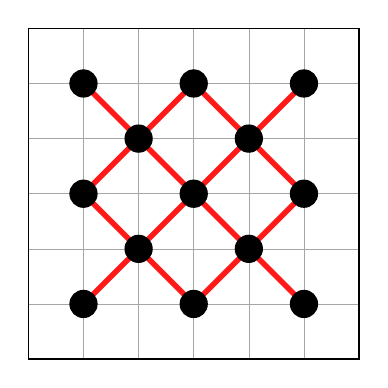
\begin{tikzpicture}[scale=0.7]
        \draw[very thin, gray!70] (0,0) grid (6,6);   
        
        \draw[red!90, line width=2pt] (1,3) -- (3,1);
        \draw[red!90, line width=2pt] (1,5) -- (5,1);
        \draw[red!90, line width=2pt] (5,3) -- (3,5);
        
        \draw[red!90, line width=2pt] (1,1) -- (5,5);
        \draw[red!90, line width=2pt] (3,1) -- (5,3);
        \draw[red!90, line width=2pt] (1,3) -- (3,5);

        %pontos normais     
        \filldraw[black] (1,1) circle (7pt);
        \filldraw[black] (3,1) circle (7pt);
        \filldraw[black] (5,1) circle (7pt);
        \filldraw[black] (2,2) circle (7pt);
        \filldraw[black] (4,2) circle (7pt);

        \filldraw[black] (1,3) circle (7pt);
        \filldraw[black] (3,3) circle (7pt);
        \filldraw[black] (5,3) circle (7pt);
        \filldraw[black] (2,4) circle (7pt);
        \filldraw[black] (4,4) circle (7pt);

        \filldraw[black] (1,5) circle (7pt);
        \filldraw[black] (3,5) circle (7pt);
        \filldraw[black] (5,5) circle (7pt);
        \draw[black, line width=0.5pt] (0,0) rectangle (6,6);

    \end{tikzpicture}
    %2
    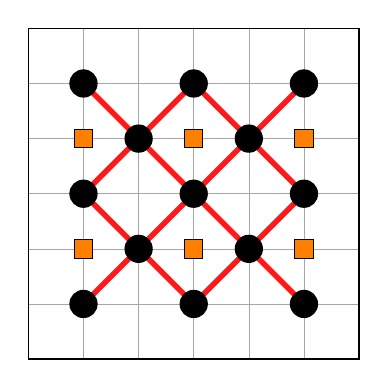
\begin{tikzpicture}[scale=0.7]
        \tikzset{
            ret/.style={
                draw,
                fill=#1,
                minimum width=0.1cm,
                minimum height=0.1cm
            }
        }
        \draw[very thin, gray!70] (0,0) grid (6,6);   

        \draw[red!90, line width=2pt] (1,3) -- (3,1);
        \draw[red!90, line width=2pt] (1,5) -- (5,1);
        \draw[red!90, line width=2pt] (5,3) -- (3,5);
        
        \draw[red!90, line width=2pt] (1,1) -- (5,5);
        \draw[red!90, line width=2pt] (3,1) -- (5,3);
        \draw[red!90, line width=2pt] (1,3) -- (3,5);


        %pontos normais     
        \filldraw[black] (1,1) circle (7pt);
        \filldraw[black] (3,1) circle (7pt);
        \filldraw[black] (5,1) circle (7pt);
        \filldraw[black] (2,2) circle (7pt);
        \filldraw[black] (4,2) circle (7pt);

        \filldraw[black] (1,3) circle (7pt);
        \filldraw[black] (3,3) circle (7pt);
        \filldraw[black] (5,3) circle (7pt);
        \filldraw[black] (2,4) circle (7pt);
        \filldraw[black] (4,4) circle (7pt);

        \filldraw[black] (1,5) circle (7pt);
        \filldraw[black] (3,5) circle (7pt);
        \filldraw[black] (5,5) circle (7pt);

        \node[ret=cor_orange] at (1,2) {};
        \node[ret=cor_orange] at (3,2) {};
        \node[ret=cor_orange] at (5,2) {};
        \node[ret=cor_orange] at (1,4) {};
        \node[ret=cor_orange] at (3,4) {};
        \node[ret=cor_orange] at (5,4) {};

        \draw[black, line width=0.5pt] (0,0) rectangle (6,6);

    \end{tikzpicture}
    %3
    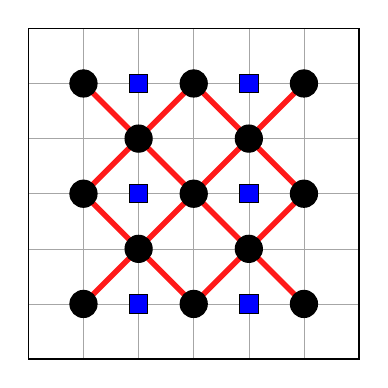
\begin{tikzpicture}[scale=0.7]
        \tikzset{
            ret/.style={
                draw,
                fill=#1,
                minimum width=0.1cm,
                minimum height=0.1cm
            }
        }
        \draw[very thin, gray!70] (0,0) grid (6,6);   

        \draw[red!90, line width=2pt] (1,3) -- (3,1);
        \draw[red!90, line width=2pt] (1,5) -- (5,1);
        \draw[red!90, line width=2pt] (5,3) -- (3,5);
        
        \draw[red!90, line width=2pt] (1,1) -- (5,5);
        \draw[red!90, line width=2pt] (3,1) -- (5,3);
        \draw[red!90, line width=2pt] (1,3) -- (3,5);


        %pontos normais     
        \filldraw[black] (1,1) circle (7pt);
        \filldraw[black] (3,1) circle (7pt);
        \filldraw[black] (5,1) circle (7pt);
        \filldraw[black] (2,2) circle (7pt);
        \filldraw[black] (4,2) circle (7pt);

        \filldraw[black] (1,3) circle (7pt);
        \filldraw[black] (3,3) circle (7pt);
        \filldraw[black] (5,3) circle (7pt);
        \filldraw[black] (2,4) circle (7pt);
        \filldraw[black] (4,4) circle (7pt);

        \filldraw[black] (1,5) circle (7pt);
        \filldraw[black] (3,5) circle (7pt);
        \filldraw[black] (5,5) circle (7pt);

        \node[ret=cor_blue] at (2,1) {};
        \node[ret=cor_blue] at (4,1) {};
        \node[ret=cor_blue] at (2,3) {};
        \node[ret=cor_blue] at (4,3) {};
        \node[ret=cor_blue] at (2,5) {};
        \node[ret=cor_blue] at (4,5) {};

        \draw[black, line width=0.5pt] (0,0) rectangle (6,6);

    \end{tikzpicture}
    \caption{À esquerda, o fio de uma variável $x_i$. Ao meio, um superconjunto arboreamente satisfeito do conjunto de pontos da esquerda que representa a valoração verdadeira para $x_i$. À direita, outro superconjunto arboreamente satisfeito que representa a valoração falsa para $x_i$. Perceba que os conjuntos de pontos adicionados para a valoração verdadeira e para a valoração falsa são disjuntos e possuem mesmo tamanho.}
\label{fig:variavel}
\end{figure}

Cada cláusula também será representada por uma coleção de pontos em $P$. Os pontos de uma cláusula $C$ são mostrados na Figura~\ref{fig:clausula}, juntamente com um conjunto independente de retângulos, indicado pelos segmentos em vermelho. Os dois cantos superiores desses dispositivo da Figura~\ref{fig:clausula} e o canto inferior direito correspondem cada um a uma das variáveis da cláusula. A ideia é que um superconjunto mínimo de $P$ arboreamente satisfeito conterá apenas dois dos quadrados rosas dos dispositivos de cada cláusula se e somente se existir uma valoração NAE para a fórmula.

\begin{figure}
    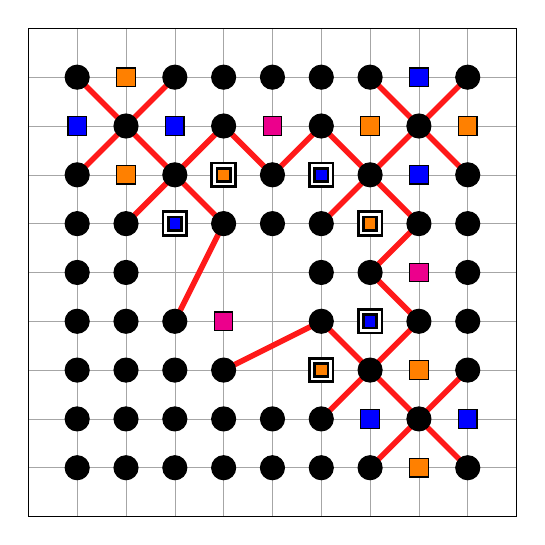
\begin{tikzpicture}[scale=0.62]
        \tikzset{
            ret/.style={
                draw,
                fill=#1,
                minimum width=0.1cm,
                minimum height=0.1cm
            },
            vipp/.style={
                draw=black,
                fill=#1,
                double,
                line width=1pt,
                double distance=0.3mm,
                minimum width=0.1cm,
                minimum height=0.1cm
            }
        }
        \draw[very thin, gray!70] (0,0) grid (10,10);   


        \draw[red!90, line width=2pt] (1,9) -- (4,6) -- (3,4);
        \draw[red!90, line width=2pt] (1,7) -- (3,9);
        \draw[red!90, line width=2pt] (2,6) -- (4,8) -- (5,7) -- (6,8) -- (8,6) -- (7,5) -- (8,4) -- (6,2);
        \draw[red!90, line width=2pt] (9,9) -- (6,6);
        \draw[red!90, line width=2pt] (7,9) -- (9,7);
        \draw[red!90, line width=2pt] (9,1) -- (6,4) -- (4,3);
        \draw[red!90, line width=2pt] (7,1) -- (9,3);


        %pontos normais     
        %1
        \filldraw[black] (1,1) circle (7pt);
        \filldraw[black] (2,1) circle (7pt);
        \filldraw[black] (3,1) circle (7pt);
        \filldraw[black] (4,1) circle (7pt);
        \filldraw[black] (5,1) circle (7pt);
        \filldraw[black] (6,1) circle (7pt);
        \filldraw[black] (7,1) circle (7pt);
        \node[ret=cor_orange] at (8,1) {};
        %\filldraw[cor1] (8,1) circle (7pt);
        \filldraw[black] (9,1) circle (7pt);

        %2
        \filldraw[black] (1,2) circle (7pt);
        \filldraw[black] (2,2) circle (7pt);
        \filldraw[black] (3,2) circle (7pt);
        \filldraw[black] (4,2) circle (7pt);
        \filldraw[black] (5,2) circle (7pt);
        \filldraw[black] (6,2) circle (7pt);
        \node[ret=cor_blue] at (7,2) {};
        %\filldraw[cor2] (7,2) circle (7pt);
        \filldraw[black] (8,2) circle (7pt);
        \node[ret=cor_blue] at (9,2) {};
        %\filldraw[cor2] (9,2) circle (7pt);

        %3
        \filldraw[black] (1,3) circle (7pt);
        \filldraw[black] (2,3) circle (7pt);
        \filldraw[black] (3,3) circle (7pt);
        \filldraw[black] (4,3) circle (7pt);
        \node[vipp=vip_orange] at (6,3) {};
        %\filldraw[cor1] (6,3) circle (7pt); %ESPECIAL
        \filldraw[black] (7,3) circle (7pt);
        \node[ret=cor_orange] at (8,3) {};
        %\filldraw[cor1] (8,3) circle (7pt);
        \filldraw[black] (9,3) circle (7pt);

        %4
        \filldraw[black] (1,4) circle (7pt);
        \filldraw[black] (2,4) circle (7pt);
        \filldraw[black] (3,4) circle (7pt);
        \node[ret=vip] at (4,4) {};
        %\filldraw[magenta] (4,4) circle (7pt);
        \filldraw[black] (6,4) circle (7pt);
        \node[vipp=cor_blue] at (7,4) {};
        %\filldraw[cor2] (7,4) circle (7pt);
        \filldraw[black] (8,4) circle (7pt);
        \filldraw[black] (9,4) circle (7pt);

        %5
        \filldraw[black] (1,5) circle (7pt);
        \filldraw[black] (2,5) circle (7pt);
        \filldraw[black] (6,5) circle (7pt);
        \filldraw[black] (7,5) circle (7pt);
        \node[ret=vip] at (8,5) {};
        %\filldraw[magenta] (8,5) circle (7pt);
        \filldraw[black] (9,5) circle (7pt);

        %6
        \filldraw[black] (1,6) circle (7pt);
        \filldraw[black] (2,6) circle (7pt);
        \node[vipp=vip_blue] at (3,6) {};
        %\filldraw[cor2] (3,6) circle (7pt); %ESPECIAL
        \filldraw[black] (4,6) circle (7pt);
        \filldraw[black] (5,6) circle (7pt);
        \filldraw[black] (6,6) circle (7pt);
        \node[vipp=vip_orange] at (7,6) {};
        %\filldraw[cor1] (7,6) circle (7pt); %ESPECIAL
        \filldraw[black] (8,6) circle (7pt);
        \filldraw[black] (9,6) circle (7pt);

        %7
        \filldraw[black] (1,7) circle (7pt);
        \node[ret=cor_orange] at (2,7) {};
        %\filldraw[cor1] (2,7) circle (7pt);
        \filldraw[black] (3,7) circle (7pt);
        \node[vipp=vip_orange] at (4,7) {};
        %\filldraw[cor1] (4,7) circle (7pt); %ESPECIAL
        \filldraw[black] (5,7) circle (7pt);
        \node[vipp=vip_blue] at (6,7) {};
        %\filldraw[cor2] (6,7) circle (7pt); %ESPECIAL
        \filldraw[black] (7,7) circle (7pt);
        \node[ret=vip_blue] at (8,7) {};
        %\filldraw[cor2] (8,7) circle (7pt);
        \filldraw[black] (9,7) circle (7pt);

        %8
        \node[ret=cor_blue] at (1,8) {};
        %\filldraw[cor2] (1,8) circle (7pt);
        \filldraw[black] (2,8) circle (7pt);
        \node[ret=cor_blue] at (3,8) {};
        %\filldraw[cor2] (3,8) circle (7pt);
        \filldraw[black] (4,8) circle (7pt);
        \node[ret=vip] at (5,8) {};
        %\filldraw[magenta] (5,8) circle (7pt);
        \filldraw[black] (6,8) circle (7pt);
        \node[ret=cor_orange] at (7,8) {};
        %\filldraw[cor1] (7,8) circle (7pt);
        \filldraw[black] (8,8) circle (7pt);
        \node[ret=cor_orange] at (9,8) {};
        %\filldraw[cor1] (9,8) circle (7pt);

        %9
        \filldraw[black] (1,9) circle (7pt);
        \node[ret=cor_orange] at (2,9) {};
        %\filldraw[cor1] (2,9) circle (7pt);
        \filldraw[black] (3,9) circle (7pt);
        \filldraw[black] (4,9) circle (7pt);
        \filldraw[black] (5,9) circle (7pt);
        \filldraw[black] (6,9) circle (7pt);
        \filldraw[black] (7,9) circle (7pt);
        \node[ret=cor_blue] at (8,9) {};
        %\filldraw[cor2] (8,9) circle (7pt);
        \filldraw[black] (9,9) circle (7pt);

        \draw[black, line width=0.5pt] (0,0) rectangle (10,10);

    \end{tikzpicture}
    \caption{Note que a única maneira de apenas adicionar dois dos três pontos indicados por retângulos rosas é com uma valoração verdadeira e outra falsa dentre as 3 valorações. Os retângulos laranjas/azuis destacados são aqueles relacionados aos retângulos rosa.}
\label{fig:clausula}
\end{figure}

Resta agora conectar as variáveis às cláusulas onde elas ocorrem. Isso é feito a partir de um desenho do grafo bipartido com variáveis de um lado e cláusulas de outro, e uma aresta ligando cada variável a cada cláusula em que ela ocorra. Por exemplo, para a instância com 5 variáveis $x_1,\ldots,x_5$ e as cláusulas $C_1 = x_1 \land x_2 \land x_4$ e $C_2 = x_3 \land x_4 \land x_5$ consideremos o desenho da Figura (ainda não feita/grafo bipartido).

Baseado neste desenho e usando dispositivos para alterar a paridade da linha dos quadrados em laranja ou em azul e para cruzar fios que estão apresentados na Figura~\ref{fig:pulo}, é possível obter o conjunto de pontos representado na Figura~\ref{fig:final}. É fácil notar que encontrar o menor superconjunto arboreamente satisfeito desse conjunto implica em encontrar uma valoração NAE para a fórmula. 

\begin{figure}
    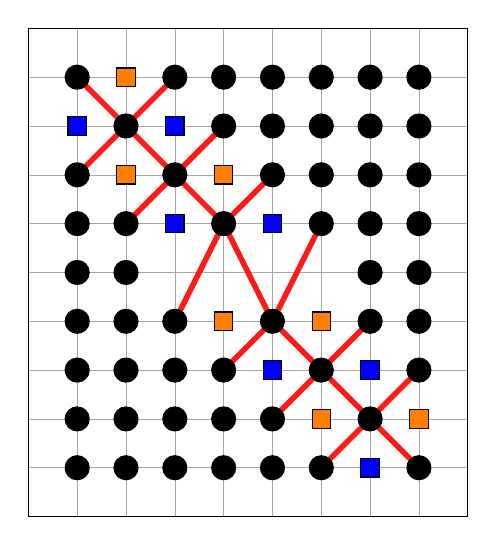
\begin{tikzpicture}[scale=0.62]
        \tikzset{
            ret/.style={
                draw,
                fill=#1,
                minimum width=0.1cm,
                minimum height=0.1cm
            }
        }
        \draw[very thin, gray!70] (0,0) grid (9,10);   

        \draw[red!90, line width=2pt] (1,9) -- (4,6) -- (5,4) -- (8,1);
        \draw[red!90, line width=2pt] (1,7) -- (3,9);
        \draw[red!90, line width=2pt] (2,6) -- (4,8);
        \draw[red!90, line width=2pt] (3,4) -- (4,6) -- (5,7);
        \draw[red!90, line width=2pt] (4,3) -- (5,4) -- (6,6);
        \draw[red!90, line width=2pt] (5,2) -- (7,4);
        \draw[red!90, line width=2pt] (6,1) -- (8,3);

        \foreach \y in {1,2,3,4,5,6,7,9} { %PONTOS PRETOS
            \filldraw[black] (1,\y) circle (7pt);
        }
        \foreach \y in {1,2,3,4,5,6,8} { %PONTOS PRETOS
            \filldraw[black] (2,\y) circle (7pt);
        }
        \foreach \y in {1,2,3,4,7,9} { %PONTOS PRETOS
            \filldraw[black] (3,\y) circle (7pt);
        }
        \foreach \y in {1,2,3,6,8,9} { %PONTOS PRETOS
            \filldraw[black] (4,\y) circle (7pt);
        }
        \foreach \y in {1,2,4,7,8,9} { %PONTOS PRETOS
            \filldraw[black] (5,\y) circle (7pt);
        }
        \foreach \y in {1,3,6,7,8,9} { %PONTOS PRETOS
            \filldraw[black] (6,\y) circle (7pt);
        }
        \foreach \y in {2,4,5,6,7,8,9} { %PONTOS PRETOS
            \filldraw[black] (7,\y) circle (7pt);
        }
        \foreach \y in {1,3,4,5,6,7,8,9} { %PONTOS PRETOS
            \filldraw[black] (8,\y) circle (7pt);
        }

        \node[ret=cor_orange] at (2,7) {};
        \node[ret=cor_orange] at (2,9) {};
        \node[ret=cor_orange] at (4,4) {};
        \node[ret=cor_orange] at (4,7) {};
        \node[ret=cor_orange] at (6,2) {};
        \node[ret=cor_orange] at (6,4) {};
        \node[ret=cor_orange] at (8,2) {};
        \node[ret=cor_blue] at (1,8) {};
        \node[ret=cor_blue] at (3,8) {};
        \node[ret=cor_blue] at (3,6) {};
        \node[ret=cor_blue] at (5,6) {};
        \node[ret=cor_blue] at (5,3) {};
        \node[ret=cor_blue] at (7,3) {};
        \node[ret=cor_blue] at (7,1) {};

        \draw[black, line width=0.5pt] (0,0) rectangle (9,10);

    \end{tikzpicture}
    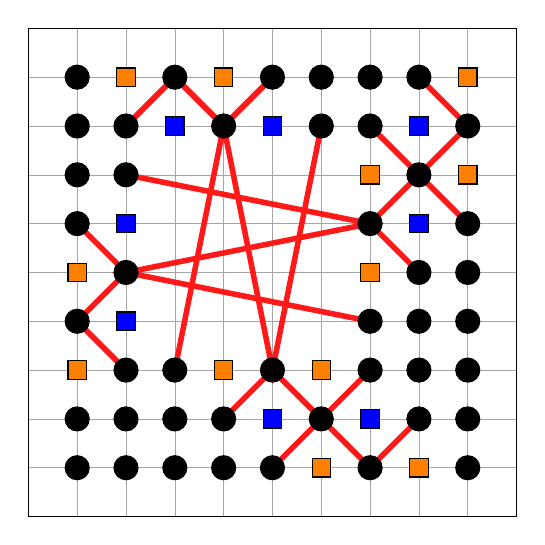
\begin{tikzpicture}[scale=0.62]
        \tikzset{
            ret/.style={
                draw,
                fill=#1,
                minimum width=0.1cm,
                minimum height=0.1cm
            }
        }
        \draw[very thin, gray!70] (0,0) grid (10,10);   


        \draw[red!90, line width=2pt] (2,3) -- (1,4) -- (2,5) -- (1,6);
        \draw[red!90, line width=2pt] (7,4) -- (2,5) -- (7,6) -- (2,7);
        \draw[red!90, line width=2pt] (3,3) -- (4,8) --(5,3) -- (6,8);
        \draw[red!90, line width=2pt] (4,2) -- (5,3) -- (6,2) -- (7,3);
        \draw[red!90, line width=2pt] (5,1) -- (6,2) -- (7,1) -- (8,2);
        \draw[red!90, line width=2pt] (2,8) -- (3,9) -- (4,8) -- (5,9);
        \draw[red!90, line width=2pt] (2,8) -- (3,9) -- (4,8) -- (5,9);
        \draw[red!90, line width=2pt] (8,5) -- (7,6) -- (9,8) -- (8,9);
        \draw[red!90, line width=2pt] (9,6) -- (7,8);

        \foreach \y in {1,2,4,6,7,8,9} { %PONTOS PRETOS
            \filldraw[black] (1,\y) circle (7pt);
        }
        \foreach \y in {1,2,3,5,7,8} { %PONTOS PRETOS
            \filldraw[black] (2,\y) circle (7pt);
        }
        \foreach \y in {1,2,3,9} { %PONTOS PRETOS
            \filldraw[black] (3,\y) circle (7pt);
        }
        \foreach \y in {1,2,8} { %PONTOS PRETOS
            \filldraw[black] (4,\y) circle (7pt);
        }
        \foreach \y in {1,3,9} { %PONTOS PRETOS
            \filldraw[black] (5,\y) circle (7pt);
        }
        \foreach \y in {2,8,9} { %PONTOS PRETOS
            \filldraw[black] (6,\y) circle (7pt);
        }
        \foreach \y in {1,3,4,6,8,9} { %PONTOS PRETOS
            \filldraw[black] (7,\y) circle (7pt);
        }
        \foreach \y in {2,3,4,5,7,9} { %PONTOS PRETOS
            \filldraw[black] (8,\y) circle (7pt);
        }
        \foreach \y in {1,2,3,4,5,6,8} { %PONTOS PRETOS
            \filldraw[black] (9,\y) circle (7pt);
        }

        \node[ret=cor_orange] at (1,3) {};
        \node[ret=cor_orange] at (1,5) {};
        \node[ret=cor_orange] at (2,9) {};
        \node[ret=cor_orange] at (4,3) {};
        \node[ret=cor_orange] at (4,9) {};
        \node[ret=cor_orange] at (6,1) {};
        \node[ret=cor_orange] at (6,3) {};
        \node[ret=cor_orange] at (7,5) {};
        \node[ret=cor_orange] at (7,7) {};
        \node[ret=cor_orange] at (8,1) {};
        \node[ret=cor_orange] at (9,7) {};
        \node[ret=cor_orange] at (9,9) {};
        \node[ret=cor_blue] at (2,4) {};
        \node[ret=cor_blue] at (2,6) {};
        \node[ret=cor_blue] at (3,8) {};
        \node[ret=cor_blue] at (5,2) {};
        \node[ret=cor_blue] at (5,8) {};
        \node[ret=cor_blue] at (7,2) {};
        \node[ret=cor_blue] at (8,6) {};
        \node[ret=cor_blue] at (8,8) {};


        \draw[black, line width=0.5pt] (0,0) rectangle (10,10);

    \end{tikzpicture}
    \caption{À esquerda, um salto que tem como finalidade alternar a paridade ou fazer uma negação. À direita, um adaptador, onde dois fios de variáveis se cruzam sem interagir entre si.}
\label{fig:pulo}
\end{figure}

\begin{figure}
    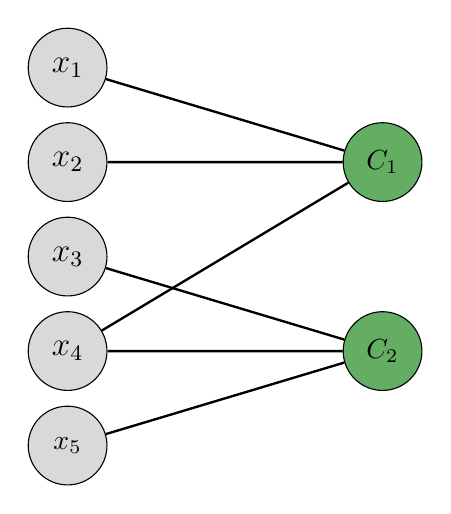
\begin{tikzpicture}[scale=0.8, node distance=2cm, every node/.style={circle, draw, minimum size=10mm, font=\sffamily}]
        
        % Definindo os nós
        \node (x1) at (0, 3) [fill=gray!30] {\large$x_1$};
        \node (x2) at (0, 1.5) [fill=gray!30] {\large$x_2$};
        \node (x3) at (0, 0) [fill=gray!30] {\large$x_3$};
        \node (x4) at (0, -1.5) [fill=gray!30] {\large$x_4$};
        \node (x5) at (0, -3) [fill=gray!30] {$x_5$};
    
        \node (c1) at (5, 1.5) [fill=ForestGreen!70] {$C_1$};
        \node (c2) at (5, -1.5) [fill=ForestGreen!70] {$C_2$};

        \draw[line width=0.03cm] (x1) -- (c1) -- (x2);
        \draw[line width=0.03cm] (c1) -- (x4);

        \draw[line width=0.03cm] (x3) -- (c2) -- (x4);
        \draw[line width=0.03cm] (c2) -- (x5);
    
    
    \end{tikzpicture}    
\caption{Grafo bipartido com as variáveis $x_1,\ldots,x_5$ de um lado e as cláusulas $C_1,C_2$ de outro.}
\label{fig:nao-planar}
\end{figure}

\begin{comment}
    \begin{figure}
        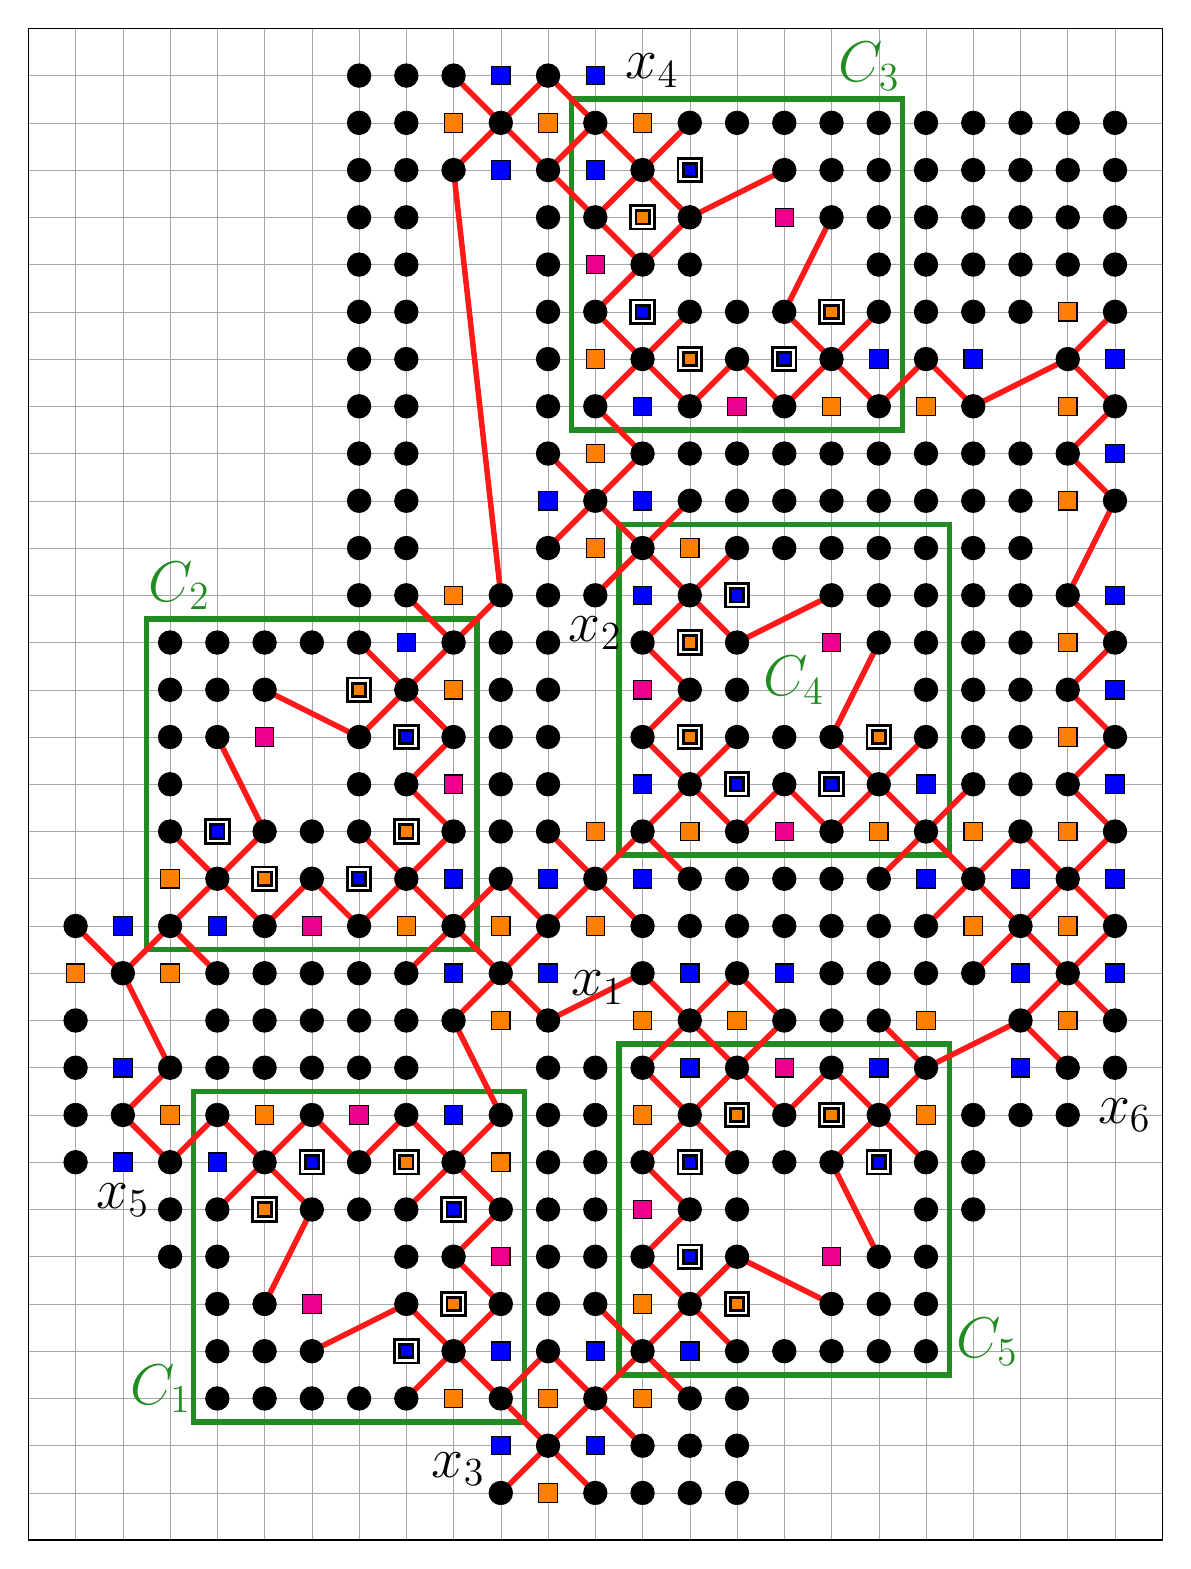
\begin{tikzpicture}[scale=0.6]
            \tikzset{
                ret/.style={
                    draw,
                    fill=#1,
                    minimum width=0.1cm,
                    minimum height=0.1cm
                },
                vipp/.style={
                    draw=black,
                    fill=#1,
                    double,
                    line width=1pt,
                    double distance=0.3mm,
                    minimum width=0.1cm,
                    minimum height=0.1cm
                }
            }
            
            \draw[very thin, gray!70] (0,0) grid (24,32); 
            
            \draw[ForestGreen,line width=0.07cm] (3.5,2.5) rectangle (10.5,9.5);
            \draw[ForestGreen,line width=0.07cm] (2.5,12.5) rectangle (9.5,19.5);
            \draw[ForestGreen,line width=0.07cm] (12.5,3.5) rectangle (19.5,10.5);
            \draw[ForestGreen,line width=0.07cm] (12.5,14.5) rectangle (19.5,21.5);
            \draw[ForestGreen,line width=0.07cm] (11.5,23.5) rectangle (18.5,30.5);

            \draw[red!90, line width=2pt] (1,13) -- (2,12) -- (3,10) -- (2,9) -- (3,8) -- (4,9) -- (5,8) -- (6,9);
            \draw[red!90, line width=2pt] (5,8) -- (6,7) -- (5,5);
            \draw[red!90, line width=2pt] (3,13) -- (4,12);
            \draw[red!90, line width=2pt] (2,12) -- (3,13) -- (4,14) -- (5,15) -- (4,17);
            \draw[red!90, line width=2pt] (4,14) -- (5,13) -- (6,14) -- (7,13) -- (9,15) -- (8,16) -- (9,17) -- (8,18) -- (7,17) -- (5,18);
            \draw[red!90, line width=2pt] (8,18) -- (9,17);
            \draw[red!90, line width=2pt] (9,19) -- (10,20) -- (9,29) -- (10,30) -- (11,29);
            \draw[red!90, line width=2pt] (9,31) -- (10,30) -- (11,31) -- (14,28) -- (16,29);
            \draw[red!90, line width=2pt] (14,28) -- (13,27) -- (12,26) -- (13,25) -- (12,24) -- (13,23) -- (12,22) -- (13,21) -- (12,20);
            \draw[red!90, line width=2pt] (11,21) -- (12,22) -- (11,23);

            \draw[red!90, line width=2pt] (7,19) -- (8,18) -- (9,19);

            \draw[red!90, line width=2pt] (10,1) -- (11,2) -- (8,5);
            \draw[red!90, line width=2pt] (8,3) -- (10,5) -- (9,6) -- (10,7) -- (9,8) -- (10,9) -- (9,11) -- (10,12) -- (9,13) -- (8,14) --(7,15);

            \draw[red!90, line width=2pt] (8,5) -- (6,4);

            \draw[red!90, line width=2pt] (6,9) -- (7,8) -- (8,9) -- (9,8);

            \draw[red!90, line width=2pt] (11,11) -- (10,12) -- (15,17);
            \draw[red!90, line width=2pt] (13,21) -- (14,20) -- (13,19) -- (14,18) -- (13,17) -- (14,16);

            \draw[red!90, line width=2pt] (14,20) -- (15,19) -- (17,20);
            \draw[red!90, line width=2pt] (17,28) -- (16,26) -- (17,25) -- (16,24) -- (15,25) -- (14,24) -- (13,25);

            \draw[red!90, line width=2pt] (18,26) -- (17,25) -- (18,24) -- (19,25) -- (20,24) -- (22,25) -- (23,26);

            \draw[red!90, line width=2pt] (22,25) -- (23,24) -- (22,23) -- (23,22) -- (22,20) -- (23,19) -- (22,18) -- (23,17) -- (22,16) -- (23,15) -- (22,14) -- (23,13) -- (22,12) -- (23,11);

            \draw[red!90, line width=2pt] (22,10) -- (21,11) -- (22,12) -- (21,13) -- (20,14) -- (21,15) -- (22,14); 
            \draw[red!90, line width=2pt] (22,14) -- (21,13) -- (17,17); 
            \draw[red!90, line width=2pt] (19,17) -- (18,16) -- (17,15) -- (16,16) -- (15,15) -- (14,16); 

            \draw[red!90, line width=2pt] (21,11) -- (19,10) -- (18,9) -- (19,8);
            \draw[red!90, line width=2pt] (18,6) -- (17,8) -- (18,9) -- (17,10) -- (16,9) -- (15,10) -- (14,9) -- (15,8);

            \draw[red!90, line width=2pt] (15,10) -- (14,11) -- (13,12) -- (11,11); 

            \draw[red!90, line width=2pt] (14,11) -- (13,10) -- (14,9) -- (13,8) -- (14,7) -- (13,6) -- (14,5) -- (15,6) -- (17,5);

            \draw[red!90, line width=2pt] (12,1) -- (11,2) -- (12,3) -- (13,4) -- (15,6); 

            \draw[red!90, line width=2pt] (13,2) -- (12,3) -- (11,4) -- (10,3);

            \draw[red!90, line width=2pt] (13,4) -- (12,5);
            \draw[red!90, line width=2pt] (9,19) -- (8,20);
            \draw[red!90, line width=2pt] (3,15) -- (4,14);
            \draw[red!90, line width=2pt] (4,7) -- (5,8);
            \draw[red!90, line width=2pt] (13,4) -- (14,3);

            \draw[red!90, line width=2pt] (20,14) -- (19,13);
            \draw[red!90, line width=2pt] (21,13) -- (20,12);
            \draw[red!90, line width=2pt] (13,13) -- (11,15);
            \draw[red!90, line width=2pt] (14,14) -- (13,15);
            \draw[red!90, line width=2pt] (14,11) -- (15,12) -- (16,11) -- (15,10);
            \draw[red!90, line width=2pt] (11,13) -- (10,14) -- (9,13);
            \draw[red!90, line width=2pt] (13,21) -- (14,22);
            \draw[red!90, line width=2pt] (17,17) -- (18,19);
            \draw[red!90, line width=2pt] (13,27) -- (11,29) -- (12,30);
            \draw[red!90, line width=2pt] (12,28) -- (14,30);
            \draw[red!90, line width=2pt] (14,5) -- (15,4);
            \draw[red!90, line width=2pt] (14,20) -- (15,21);
            \draw[red!90, line width=2pt] (18,14) -- (19,15) -- (20,16);
            \draw[red!90, line width=2pt] (13,25) -- (14,26);



            \draw[red!90, line width=2pt] (8,7) -- (9,8);
            \draw[red!90, line width=2pt] (9,13) -- (8,12);
            \draw[red!90, line width=2pt] (19,10) -- (18,11);
            
            %vamos fazer por colunas
            %coluna 2
            \foreach \y in {8, 9, 10, 11, 13} {
                \filldraw[black] (1,\y) circle (7pt);
            }
            \foreach \y in {12} { % LARANJAS
                \node[ret=cor_orange] at (1,\y) {};
            }

            %coluna 3
            \foreach \y in {9, 12} {
                \filldraw[black] (2,\y) circle (7pt);
            }
            \foreach \y in {8, 10, 13} {
                \node[ret=cor_blue] at (2,\y) {};
            }

            %coluna 4
            \filldraw[black] (3,6) circle (7pt);
            \filldraw[black] (3,7) circle (7pt);
            \filldraw[black] (3,8) circle (7pt);
            \node[ret=cor_orange] at (3,9) {};
            \filldraw[black] (3,10) circle (7pt);
            \node[ret=cor_orange] at (3,12) {};
            \filldraw[black] (3,13) circle (7pt);
            \node[ret=cor_orange] at (3,14) {};
            \filldraw[black] (3,15) circle (7pt);
            \filldraw[black] (3,16) circle (7pt);
            \filldraw[black] (3,17) circle (7pt);
            \filldraw[black] (3,18) circle (7pt);
            \filldraw[black] (3,19) circle (7pt);

            %coluna 5
            \node[ret=cor_blue] at (4,8) {};
            \filldraw[black] (4,3) circle (7pt);
            \filldraw[black] (4,4) circle (7pt);
            \filldraw[black] (4,5) circle (7pt);
            \filldraw[black] (4,6) circle (7pt);
            \filldraw[black] (4,7) circle (7pt);
            \filldraw[black] (4,9) circle (7pt);
            \filldraw[black] (4,10) circle (7pt);
            \filldraw[black] (4,11) circle (7pt);
            \filldraw[black] (4,12) circle (7pt);
            \node[ret=cor_blue] at (4,13) {};
            \filldraw[black] (4,14) circle (7pt);
            \node[vipp=vip_blue] at (4,15) {};
            \filldraw[black] (4,17) circle (7pt);
            \filldraw[black] (4,18) circle (7pt);
            \filldraw[black] (4,19) circle (7pt);

            %coluna 6
            \foreach \y in {9} { % LARANJAS
                \node[ret=cor_orange] at (5,\y) {};
            }
            \foreach \y in {3,4,5, 8, 10, 11, 12, 13, 15, 18, 19} { %PONTOS PRETOS
                \filldraw[black] (5,\y) circle (7pt);
            }
            \node[vipp=vip_orange] at (5,7) {};
            \node[vipp=vip_orange] at (5,14) {};
            \node[ret=vip] at (5,17) {};

            %coluna 7
            \foreach \y in {3, 4, 7,9,10,11,12,14, 15, 19} { %PONTOS PRETOS
                \filldraw[black] (6,\y) circle (7pt);
            }
            \node[ret=vip] at (6,5) {};
            \node[ret=vip] at (6,13) {};
            \node[vipp=vip_blue] at (6,8) {};

            %coluna 8
            \foreach \y in {3, 7, 8,10,11,12, 13, 15, 16, 17, 19, 20, 21, 22, 23, 24, 25, 26, 27, 28, 29, 30, 31} { %PONTOS PRETOS
                \filldraw[black] (7,\y) circle (7pt);
            }
            \foreach \y in {} { % AZUIS
                \node[ret=cor_blue] at (7,\y) {};
            }
            \node[ret=vip] at (7,9) {};
            \node[vipp=vip_orange] at (7,18) {};
            \node[vipp=vip_blue] at (7,14) {};

            %coluna 9
            \foreach \y in {3, 5, 6, 7, 9,10,11,12, 14, 16, 18, 20, 21, 22, 23, 24, 25, 26, 27, 28, 29, 30, 31} { %PONTOS PRETOS
                \filldraw[black] (8,\y) circle (7pt);
            }
            \foreach \y in {19} { % AZUIS
                \node[ret=cor_blue] at (8,\y) {};
            }
            \foreach \y in {13} { % LARANJAS
                \node[ret=cor_orange] at (8,\y) {};
            }
            \node[vipp=vip_orange] at (8,8) {};
            \node[vipp=vip_orange] at (8,15) {};
            \node[vipp=vip_blue] at (8,4) {};
            \node[vipp=vip_blue] at (8,17) {};
            

            %coluna 10
            \foreach \y in {4, 6, 8, 11, 13, 15, 17, 19, 29, 31} { %PONTOS PRETOS
                \filldraw[black] (9,\y) circle (7pt);
            }
            \foreach \y in {9, 12, 14} { % AZUIS
                \node[ret=cor_blue] at (9,\y) {};
            }
            \foreach \y in {3, 18, 20, 30} { % LARANJAS
                \node[ret=cor_orange] at (9,\y) {};
            }
            \node[vipp=vip_orange] at (9,5) {};
            \node[vipp=vip_blue] at (9,7) {};
            \node[ret=vip] at (9,16) {};

            %coluna 11
            \foreach \y in {1, 3, 5, 7, 9, 12, 14, 15, 16, 17, 18, 19, 20, 30} { %PONTOS PRETOS
                \filldraw[black] (10,\y) circle (7pt);
            }
            \foreach \y in {2, 4, 29, 31} { % AZUIS
                \node[ret=cor_blue] at (10,\y) {};
            }
            \foreach \y in {8, 11, 13} { % LARANJAS
                \node[ret=cor_orange] at (10,\y) {};
            }
            \node[ret=vip] at (10,6) {};

            %coluna 12
            \foreach \y in {2, 4, 5, 6, 7, 8, 9, 10, 11, 13, 15, 16, 17, 18, 19, 20, 21, 23, 24, 25, 26, 27, 28, 29, 31} { %PONTOS PRETOS
                \filldraw[black] (11,\y) circle (7pt);
            }
            \foreach \y in {12, 14, 22} { % AZUIS
                \node[ret=cor_blue] at (11,\y) {};
            }
            \foreach \y in {1, 3, 30} { % LARANJAS
                \node[ret=cor_orange] at (11,\y) {};
            }

            %coluna 13
            \foreach \y in {1, 3, 5, 6, 7, 8, 9, 10, 14, 20, 22, 24, 26, 28, 30} { %PONTOS PRETOS
                \filldraw[black] (12,\y) circle (7pt);
            }
            \foreach \y in {2, 4, 29, 31} { % AZUIS
                \node[ret=cor_blue] at (12,\y) {};
            }
            \foreach \y in {13, 15, 21, 23, 25} { % LARANJAS
                \node[ret=cor_orange] at (12,\y) {};
            }
            \node[ret=vip] at (12,27) {};

            %coluna 14
            \foreach \y in {1, 2, 4, 6, 8, 10, 12, 13, 15, 17, 19, 21, 23, 25, 27, 29} { %PONTOS PRETOS
                \filldraw[black] (13,\y) circle (7pt);
            }
            \foreach \y in {14, 16, 20, 22, 24} { % AZUIS
                \node[ret=cor_blue] at (13,\y) {};
            }
            \foreach \y in {3, 5, 9, 11, 30} { % LARANJAS
                \node[ret=cor_orange] at (13,\y) {};
            }
            \node[vipp=vip_blue] at (13,26) {};
            \node[vipp=vip_orange] at (13,28) {};
            \node[ret=vip] at (13,7) {};
            \node[ret=vip] at (13,18) {};

            %coluna 15
            \foreach \y in {1,2,3,5, 7, 9, 11, 13, 14, 16, 18, 20, 22, 23, 24, 26, 27, 28,  30} { %PONTOS PRETOS
                \filldraw[black] (14,\y) circle (7pt);
            }
            \foreach \y in {4, 10, 12} { % AZUIS
                \node[ret=cor_blue] at (14,\y) {};
            }
            \foreach \y in {15, 21} { % LARANJAS
                \node[ret=cor_orange] at (14,\y) {};
            }
            \node[vipp=vip_blue] at (14,6) {};
            \node[vipp=vip_blue] at (14,8) {};
            \node[vipp=vip_blue] at (14,29) {};
            \node[vipp=vip_orange] at (14,17) {};
            \node[vipp=vip_orange] at (14,19) {};
            \node[vipp=vip_orange] at (14,25) {};

            %coluna 16
            \foreach \y in {1,2,3,4, 6, 7, 8, 10, 12, 13, 14, 15, 17, 18, 19, 21, 22, 23, 25, 26, 30} { %PONTOS PRETOS
                \filldraw[black] (15,\y) circle (7pt);
            }
            \foreach \y in {11} { % LARANJAS
                \node[ret=cor_orange] at (15,\y) {};
            }
            \node[vipp=vip_orange] at (15,5) {};
            \node[vipp=vip_orange] at (15,9) {};
            \node[vipp=vip_blue] at (15,16) {};
            \node[vipp=vip_blue] at (15,20) {};
            \node[ret=vip] at (15,24) {};

            %coluna 17
            \foreach \y in {4, 8, 9, 11, 13, 14, 16, 17, 21, 22, 23, 24, 26, 29,30} { %PONTOS PRETOS
                \filldraw[black] (16,\y) circle (7pt);
            }
            \foreach \y in {12} { % AZUIS
                \node[ret=cor_blue] at (16,\y) {};
            }
            \node[vipp=vip_blue] at (16,25) {};
            \node[ret=vip] at (16,10) {};
            \node[ret=vip] at (16,15) {};
            \node[ret=vip] at (16,28) {};

            %coluna 18
            \foreach \y in {4, 5, 8, 10, 11, 12, 13, 14, 15, 17, 20, 21, 22, 23, 25, 28, 29, 30} { %PONTOS PRETOS
                \filldraw[black] (17,\y) circle (7pt);
            }
            \foreach \y in {24} { % AZUIS
                \node[ret=cor_orange] at (17,\y) {};
            }
            \node[ret=vip] at (17,6) {};
            \node[ret=vip] at (17,19) {};
            \node[vipp=vip_blue] at (17,16) {};
            \node[vipp=vip_orange] at (17,9) {};
            \node[vipp=vip_orange] at (17,26) {};

            %coluna 19
            \foreach \y in {4, 5, 6, 9, 11, 12, 13, 14, 16, 19,20, 21, 22, 23, 24, 26,27,28,29 ,30} { %PONTOS PRETOS
                \filldraw[black] (18,\y) circle (7pt);
            }
            \foreach \y in {10, 25} { % AZUIS
                \node[ret=cor_blue] at (18,\y) {};
            }
            \foreach \y in {15} { % LARANJAS
                \node[ret=cor_orange] at (18,\y) {};
            }

            \node[vipp=vip_blue] at (18,8) {};
            \node[vipp=vip_orange] at (18,17) {};

            %coluna 20
            \foreach \y in {4, 5, 6, 7, 8, 10, 12, 13, 15, 17, 18, 19, 20, 21,22, 23, 25, 26, 27, 28, 29, 30} { %PONTOS PRETOS
                \filldraw[black] (19,\y) circle (7pt);
            }
            \foreach \y in {14, 16} { % AZUIS
                \node[ret=cor_blue] at (19,\y) {};
            }
            \foreach \y in {9, 11, 24} { % LARANJAS
                \node[ret=cor_orange] at (19,\y) {};
            }

            %coluna 21
            \foreach \y in {7,8,9, 12, 14, 16, 17, 18, 19, 20, 21, 22, 23, 24, 26, 27, 28, 29, 30} { %PONTOS PRETOS
                \filldraw[black] (20,\y) circle (7pt);
            }
            \foreach \y in {13, 15} { % LARANJAS
                \node[ret=cor_orange] at (20,\y) {};
            }
            \foreach \y in {25} { % LARANJAS
                \node[ret=cor_blue] at (20,\y) {};
            }

            %coluna 22
            \foreach \y in {9, 11, 13, 15, 16, 17, 18, 19, 20, 21, 22, 23, 26, 27, 28, 29, 30} { %PONTOS PRETOS
                \filldraw[black] (21,\y) circle (7pt);
            }
            \foreach \y in {10, 12, 14} { % AZUIS
                \node[ret=cor_blue] at (21,\y) {};
            }

            %coluna 23
            \foreach \y in {9, 10, 12, 14, 16, 18, 20, 23, 25, 27, 28, 29, 30} { %PONTOS PRETOS
                \filldraw[black] (22,\y) circle (7pt);
            }
            \foreach \y in {11, 13, 15, 17, 19, 22, 24, 26} { % LARANJAS
                \node[ret=cor_orange] at (22,\y) {};
            }

            %coluna 24
            \foreach \y in {10, 11, 13, 15, 17, 19, 22, 24, 26, 27, 28, 29, 30} { %PONTOS PRETOS
                \filldraw[black] (23,\y) circle (7pt);
            }
            \foreach \y in {12, 14, 16, 18, 20, 23, 25} { % AZUIS
                \node[ret=cor_blue] at (23,\y) {};
            }
            \foreach \y in {} { % LARANJAS
                \node[ret=cor_orange] at (23,\y) {};
            }

            \node at (2.8,3.2) [text=ForestGreen] {\huge$C_1$};
            \node at (3.2,20.2) [text=ForestGreen] {\huge$C_2$};
            \node at (20.3,4.2) [text=ForestGreen] {\huge$C_5$};
            \node at (16.2,18.2) [text=ForestGreen] {\huge$C_4$};
            \node at (17.8,31.2) [text=ForestGreen] {\huge$C_3$};
            \node at (12.05,11.7) {\huge$x_1$};
            \node at (12,19.2) {\huge$x_2$};
            \node at (23.2,9) {\huge$x_6$};
            \node at (9.1,1.5) {\huge$x_3$};
            \node at (2,7.2) {\huge$x_5$};
            \node at (13.2,31.1) {\huge$x_4$};


            \draw[black, line width=0.5pt] (0,0) rectangle (24,32);

        \end{tikzpicture}
        \caption{Representação do problema dentro do contexto de buscas múltiplas. Perceba que todas as valorações possuem mesmo custo e o menor custo só se dá quando se respeita a restrição do problema 3SAT Not-All-Equal.}
    \label{fig:final}
    \end{figure}
\end{comment}

\begin{figure}
    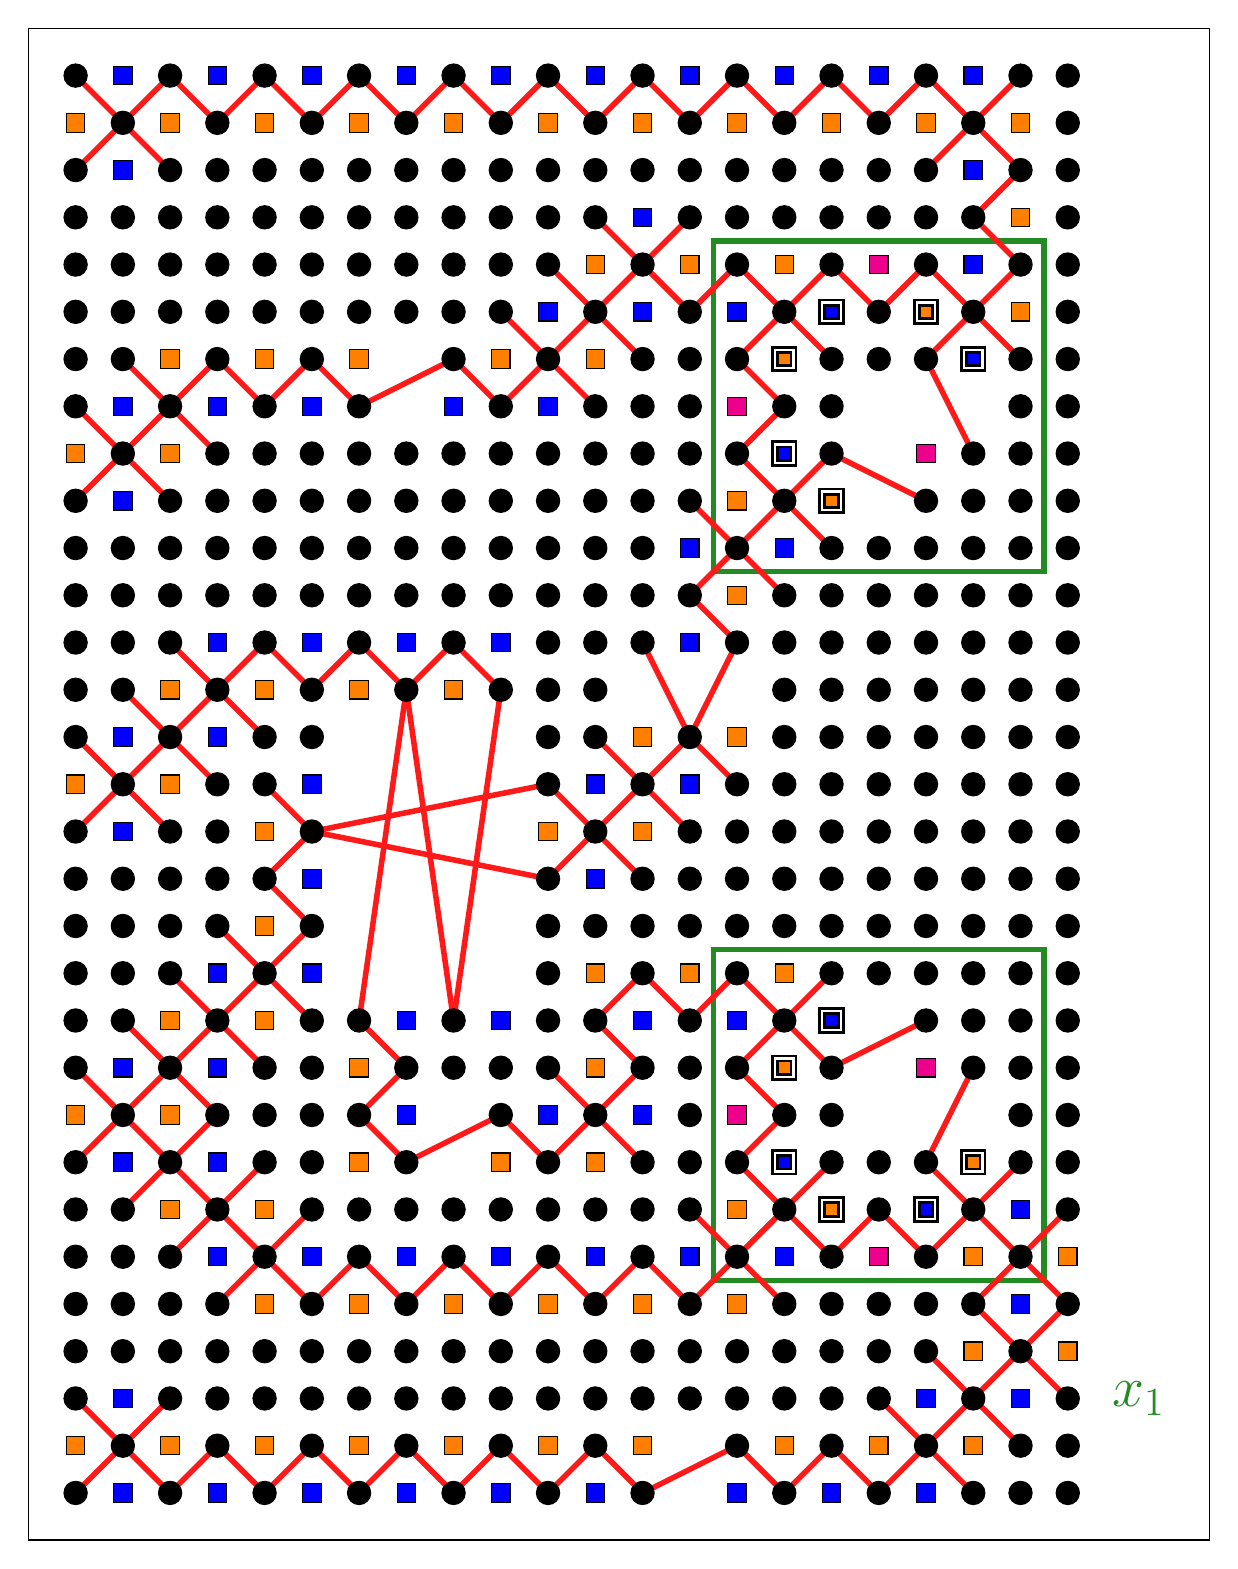
\begin{tikzpicture}[scale=0.6]
        \tikzset{
            ret/.style={
                draw,
                fill=#1,
                minimum width=0.1cm,
                minimum height=0.1cm
            },
            vipp/.style={
                draw=black,
                fill=#1,
                double,
                line width=1pt,
                double distance=0.3mm,
                minimum width=0.1cm,
                minimum height=0.1cm
            }
        }

        \draw[ForestGreen,line width=0.07cm] (14.5,27.5) rectangle (21.5,20.5);
        \draw[ForestGreen,line width=0.07cm] (14.5,12.5) rectangle (21.5,5.5);


        \draw[red!90, line width=2pt] (1,31) -- (2,30) -- (3,31) -- (4,30) -- (5,31) -- (6,30) -- (7,31) -- (8,30) -- (9,31) -- (10,30) -- (11,31) -- (12,30) -- (13,31) -- (14,30) -- (15,31) -- (16,30) -- (17,31) -- (18,30) -- (19,31) -- (20,30) -- (21,29) -- (20,28) -- (21,27) -- (20,26) -- (19,25) -- (20,23);

        \draw[red!90, line width=2pt] (1,24) -- (2,23) -- (3,24) -- (4,25) -- (5,24) -- (6,25) -- (7,24) -- (9,25) -- (10,24) -- (11,25) -- (12,26) -- (13,27) -- (14,26) -- (15,27) -- (16,26) -- (17,27) -- (18,26) -- (19,27) -- (20,26) -- (21,25);


        \draw[red!90, line width=2pt] (1,29) -- (2,30) -- (3,29);

        \draw[red!90, line width=2pt] (21,31) -- (19,29);
        \draw[red!90, line width=2pt] (2,25) -- (4,23);
        \draw[red!90, line width=2pt] (1,17) -- (3,15);
        \draw[red!90, line width=2pt] (2,18) -- (4,16);
        \draw[red!90, line width=2pt] (3,19) -- (5,17);
        
        \draw[red!90, line width=2pt] (1,22) -- (2,23) -- (3,22);
        \draw[red!90, line width=2pt] (10,26) -- (12,24);
        \draw[red!90, line width=2pt] (11,27) -- (13,25);
        \draw[red!90, line width=2pt] (13,27) -- (14,28);
        \draw[red!90, line width=2pt] (12,28) -- (14,26);
        \draw[red!90, line width=2pt] (1,10) -- (6,5) -- (7,6) -- (8,5) -- (9,6) -- (10,5) -- (11,6) -- (12,5) -- (13,6) -- (14,5) -- (17,8);
        
        \draw[red!90, line width=2pt] (1,15) -- (5,19) -- (6,18) -- (7,19) -- (8,18) -- (9,19) -- (10,18);
        
        % -- (9,10.8) -- (8,18) -- (7,11);
        \draw[red!90, line width=2pt] (9,11) -- (8,18);
        \draw[red!90, line width=2pt] (7,11) -- (8,18);
        \draw[red!90, line width=2pt] (9,11) -- (10,18);
        \draw[red!90, line width=2pt] (18,3) -- (20,1);
        \draw[red!90, line width=2pt] (19,4) -- (21,2);
        \draw[red!90, line width=2pt] (20,5) -- (22,3);
        \draw[red!90, line width=2pt] (20,5) -- (22,7);
        \draw[red!90, line width=2pt] (21,8) -- (19,6) -- (18,7) -- (17,6) -- (16,7) -- (15,6);
        
        \draw[red!90, line width=2pt] (1,3) -- (2,2) -- (3,3);
        
        \draw[red!90, line width=2pt] (1,8) -- (5,12);
        \draw[red!90, line width=2pt] (2,7) -- (4,9);
        \draw[red!90, line width=2pt] (4,5) -- (6,7);
        \draw[red!90, line width=2pt] (3,6) -- (5,8);
        \draw[red!90, line width=2pt] (11,14) -- (14,17) -- (15,19) -- (14,20) -- (17,23) -- (19,22);
        
        
        \draw[red!90, line width=2pt] (1,1) -- (2,2) -- (3,1) -- (4,2) -- (5,1) -- (6,2) -- (7,1) -- (8,2) -- (9,1) -- (10,2) -- (11,1) -- (12,2) -- (13,1) -- (15,2) -- (16,1) -- (17,2) -- (18,1) -- (19,2) -- (22,5) -- (19,8) -- (20,10);
        %\draw[red!90, line width=2pt] ();
        
        
        \draw[red!90, line width=2pt] (11,10) -- (13,8);
        \draw[red!90, line width=2pt] (11,16) -- (6,15);
        \draw[red!90, line width=2pt] (6,15) -- (11,14);



        \draw[red!90, line width=2pt] (17,12) -- (15,10) -- (16,9) -- (15,8) -- (16,7);




        \draw[red!90, line width=2pt] (2,11) -- (4,9);
        \draw[red!90, line width=2pt] (16,26) -- (17,25);
        \draw[red!90, line width=2pt] (3,12) -- (5,10);
        \draw[red!90, line width=2pt] (14,7) -- (16,5);
        \draw[red!90, line width=2pt] (7,11) -- (8,10) -- (7,9) -- (8,8) -- (10,9) -- (11,8) -- (13,10) -- (12,11) -- (13,12) -- (14,11) -- (15,12);
        
        \draw[red!90, line width=2pt] (13,14) -- (11,16);
        \draw[red!90, line width=2pt] (14,15) -- (12,17);
        \draw[red!90, line width=2pt] (14,17) -- (15,16);
        
        \draw[red!90, line width=2pt] (15,12) -- (17,10) -- (19,11);
        
        
        
        \draw[red!90, line width=2pt] (5,14) -- (6,13);
        \draw[red!90, line width=2pt] (13,19) -- (14,17);
        
        
        \draw[red!90, line width=2pt] (14,22) -- (16,20);
        \draw[red!90, line width=2pt] (17,21) -- (15,23) -- (16,24) -- (15,25) -- (16,26);
        
        
        \draw[red!90, line width=2pt] (6,13) -- (5,12);
        \draw[red!90, line width=2pt] (4,13) -- (6,11);
        \draw[red!90, line width=2pt] (5,16) -- (6,15) -- (5,14);
        
        
        
        
        %linha 1
        \foreach \y in {1,3,5,7,9,11,13,15,17,19,21,22} { %PONTOS PRETOS
            \filldraw[black] (\y,31) circle (7pt);
        }
        \foreach \y in {} { % LARANJAS
            \node[ret=cor_orange] at (\y,31) {};
        }
        \foreach \y in {2,4,6,8,10,12,14,16,18,20} { % AZUL
            \node[ret=cor_blue] at (\y,31) {};
        }

        %linha 2
        \foreach \y in {2,4,6,8,10,12,14,16,18,20,22} { %PONTOS PRETOS
            \filldraw[black] (\y,30) circle (7pt);
        }
        \foreach \y in {1,3,5,7,9,11,13,15,17,19,21} { % LARANJAS
            \node[ret=cor_orange] at (\y,30) {};
        }
        \foreach \y in {} { % AZUL
            \node[ret=cor_blue] at (\y,30) {};
        }

        %linha 3
        \foreach \y in {1,3,4,5,6,7,8,9,10,11,12,13,14,15,16,17,18,19,21,22} { %PONTOS PRETOS
            \filldraw[black] (\y,29) circle (7pt);
        }
        \foreach \y in {} { % LARANJAS
            \node[ret=cor_orange] at (\y,29) {};
        }
        \foreach \y in {2,20} { % AZUL
            \node[ret=cor_blue] at (\y,29) {};
        }

        %linha 4
        \foreach \y in {1,2,3,4,5,6,7,8,9,10,11,12,15,14,16,17,18,19,20,22} { %PONTOS PRETOS
            \filldraw[black] (\y,28) circle (7pt);
        }
        \foreach \y in {21} { % LARANJAS
            \node[ret=cor_orange] at (\y,28) {};
        }
        \foreach \y in {13} { % AZUL
            \node[ret=cor_blue] at (\y,28) {};
        }

        %linha 5
        \foreach \y in {1,2,3,4,5,6,7,8,9,10,11,13,15,17,19,21,22} { %PONTOS PRETOS
            \filldraw[black] (\y,27) circle (7pt);
        }
        \foreach \y in {12,14,16} { % LARANJAS
            \node[ret=cor_orange] at (\y,27) {};
        }
        \foreach \y in {20} { % AZUL
            \node[ret=cor_blue] at (\y,27) {};
        }
        \node[ret=vip] at (18,27) {};

        %linha 6
        \foreach \y in {1,2,3,4,5,6,7,8,9,10,12,14,16,18,20,22} { %PONTOS PRETOS
            \filldraw[black] (\y,26) circle (7pt);
        }
        \foreach \y in {21} { % LARANJAS
            \node[ret=cor_orange] at (\y,26) {};
        }
        \foreach \y in {11,13,15} { % AZUL
            \node[ret=cor_blue] at (\y,26) {};
        }
        \node[vipp=vip_blue] at (17,26) {};
        \node[vipp=vip_orange] at (19,26) {};

        %linha 7
        \foreach \y in {1,2,4,6,9,11,13,14,15,17,18,19,21,22} { %PONTOS PRETOS
            \filldraw[black] (\y,25) circle (7pt);
        }
        \foreach \y in {3,5,7,10,12} { % LARANJAS
            \node[ret=cor_orange] at (\y,25) {};
        }
        \foreach \y in {} { % AZUL
            \node[ret=cor_blue] at (\y,25) {};
        }
        \node[vipp=vip_orange] at (16,25) {};
        \node[vipp=vip_blue] at (20,25) {};

        %linha 8
        \foreach \y in {1,3,5,7,10,12,13,14,16,17,21,22} { %PONTOS PRETOS
            \filldraw[black] (\y,24) circle (7pt);
        }
        \foreach \y in {} { % LARANJAS
            \node[ret=cor_orange] at (\y,24) {};
        }
        \foreach \y in {2,4,6,9,11} { % AZUL
            \node[ret=cor_blue] at (\y,24) {};
        }
        \node[ret=vip] at (15,24) {};

        %linha 9
        \foreach \y in {2,4,5,6,7,8,9,10,11,12,13,14,15,17,20,21,22} { %PONTOS PRETOS
            \filldraw[black] (\y,23) circle (7pt);
        }
        \foreach \y in {1,3} { % LARANJAS
            \node[ret=cor_orange] at (\y,23) {};
        }
        \foreach \y in {} { % AZUL
            \node[ret=cor_blue] at (\y,23) {};
        }
        \node[vipp=vip_blue] at (16,23) {};
        \node[ret=vip] at (19,23) {};

        %linha 10
        \foreach \y in {1,3,4,5,6,7,8,9,10,11,12,13,14,16,19,20,21,22} { %PONTOS PRETOS
            \filldraw[black] (\y,22) circle (7pt);
        }
        \foreach \y in {15} { % LARANJAS
            \node[ret=cor_orange] at (\y,22) {};
        }
        \foreach \y in {2} { % AZUL
            \node[ret=cor_blue] at (\y,22) {};
        }
        \node[vipp=vip_orange] at (17,22) {};

        %linha 11
        \foreach \y in {1,2,3,4,5,6,7,8,9,10,11,12,13,15,17,18,19,20,21,22} { %PONTOS PRETOS
            \filldraw[black] (\y,21) circle (7pt);
        }
        \foreach \y in {} { % LARANJAS
            \node[ret=cor_orange] at (\y,21) {};
        }
        \foreach \y in {14,16} { % AZUL
            \node[ret=cor_blue] at (\y,21) {};
        }

        %linha 12
        \foreach \y in {1,2,3,4,5,6,7,8,9,10,11,12,13,14,16,17,18,19,20,21,22} { %PONTOS PRETOS
            \filldraw[black] (\y,20) circle (7pt);
        }
        \foreach \y in {15} { % LARANJAS
            \node[ret=cor_orange] at (\y,20) {};
        }
        \foreach \y in {} { % AZUL
            \node[ret=cor_blue] at (\y,20) {};
        }

        %linha 13
        \foreach \y in {1,2,3,5,7,9,11,12,13,15,16,17,18,19,20,21,22} { %PONTOS PRETOS
            \filldraw[black] (\y,19) circle (7pt);
        }
        \foreach \y in {} { % LARANJAS
            \node[ret=cor_orange] at (\y,19) {};
        }
        \foreach \y in {4,6,8,10,14} { % AZUL
            \node[ret=cor_blue] at (\y,19) {};
        }

        %linha 14
        \foreach \y in {1,2,4,6,8,10,11,12,16,17,18,19,20,21,22} { %PONTOS PRETOS
            \filldraw[black] (\y,18) circle (7pt);
        }
        \foreach \y in {3,5,7,9} { % LARANJAS
            \node[ret=cor_orange] at (\y,18) {};
        }
        \foreach \y in {} { % AZUL
            \node[ret=cor_blue] at (\y,18) {};
        }

        %linha 15
        \foreach \y in {1,3,5,6,11,12,14,16,17,18,19,20,21,22} { %PONTOS PRETOS
            \filldraw[black] (\y,17) circle (7pt);
        }
        \foreach \y in {13,15} { % LARANJAS
            \node[ret=cor_orange] at (\y,17) {};
        }
        \foreach \y in {2,4} { % AZUL
            \node[ret=cor_blue] at (\y,17) {};
        }

        %linha 16
        \foreach \y in {2,4,5,11,13,15,16,17,18,19,20,21,22} { %PONTOS PRETOS
            \filldraw[black] (\y,16) circle (7pt);
        }
        \foreach \y in {1,3} { % LARANJAS
            \node[ret=cor_orange] at (\y,16) {};
        }
        \foreach \y in {6,12,14} { % AZUL
            \node[ret=cor_blue] at (\y,16) {};
        }

        %linha 17
        \foreach \y in {1,3,4,6,12,14,15,16,17,18,19,20,21,22} { %PONTOS PRETOS
            \filldraw[black] (\y,15) circle (7pt);
        }
        \foreach \y in {5,11,13} { % LARANJAS
            \node[ret=cor_orange] at (\y,15) {};
        }
        \foreach \y in {2} { % AZUL
            \node[ret=cor_blue] at (\y,15) {};
        }

        %linha 18
        \foreach \y in {1,2,3,4,5,11,13,14,15,16,17,18,19,20,21,22} { %PONTOS PRETOS
            \filldraw[black] (\y,14) circle (7pt);
        }
        \foreach \y in {} { % LARANJAS
            \node[ret=cor_orange] at (\y,14) {};
        }
        \foreach \y in {6,12} { % AZUL
            \node[ret=cor_blue] at (\y,14) {};
        }

        %linha 19
        \foreach \y in {1,2,3,4,6,11,12,13,14,15,16,17,18,19,20,21,22} { %PONTOS PRETOS
            \filldraw[black] (\y,13) circle (7pt);
        }
        \foreach \y in {5} { % LARANJAS
            \node[ret=cor_orange] at (\y,13) {};
        }
        \foreach \y in {} { % AZUL
            \node[ret=cor_blue] at (\y,13) {};
        }

        %linha 20
        \foreach \y in {1,2,3,5,11,13,15,17,18,19,20,21,22} { %PONTOS PRETOS
            \filldraw[black] (\y,12) circle (7pt);
        }
        \foreach \y in {12,14,16} { % LARANJAS
            \node[ret=cor_orange] at (\y,12) {};
        }
        \foreach \y in {4,6} { % AZUL
            \node[ret=cor_blue] at (\y,12) {};
        }

        %linha 21
        \foreach \y in {1,2,4,6,7,9,11,12,14,16,19,20,21,22} { %PONTOS PRETOS
            \filldraw[black] (\y,11) circle (7pt);
        }
        \foreach \y in {3,5} { % LARANJAS
            \node[ret=cor_orange] at (\y,11) {};
        }
        \foreach \y in {8,10,13,15} { % AZUL
            \node[ret=cor_blue] at (\y,11) {};
        }
        \node[vipp=vip_blue] at (17,11) {};

        %linha 22
        \foreach \y in {1,3,5,6,8,9,10,11,13,14,15,17,20,21,22} { %PONTOS PRETOS
            \filldraw[black] (\y,10) circle (7pt);
        }
        \foreach \y in {7,12} { % LARANJAS
            \node[ret=cor_orange] at (\y,10) {};
        }
        \foreach \y in {2,4} { % AZUL
            \node[ret=cor_blue] at (\y,10) {};
        }
        \node[ret=vip] at (19,10) {};
        \node[vipp=vip_orange] at (16,10) {};

        %linha 23
        \foreach \y in {2,4,5,6,7,10,12,14,16,17,21,22} { %PONTOS PRETOS
            \filldraw[black] (\y,9) circle (7pt);
        }
        \foreach \y in {1,3} { % LARANJAS
            \node[ret=cor_orange] at (\y,9) {};
        }
        \foreach \y in {8,11,13} { % AZUL
            \node[ret=cor_blue] at (\y,9) {};
        }
        \node[ret=vip] at (15,9) {};

        %linha 24
        \foreach \y in {1,3,5,6,8,11,13,14,15,17,18,19,21,22} { %PONTOS PRETOS
            \filldraw[black] (\y,8) circle (7pt);
        }
        \foreach \y in {7,10,12} { % LARANJAS
            \node[ret=cor_orange] at (\y,8) {};
        }
        \foreach \y in {2,4} { % AZUL
            \node[ret=cor_blue] at (\y,8) {};
        }
        \node[vipp=vip_blue] at (16,8) {};
        \node[vipp=vip_orange] at (20,8) {};

        %linha 25
        \foreach \y in {1,2,4,6,7,8,9,10,11,12,13,14,16,18,20,22} { %PONTOS PRETOS
            \filldraw[black] (\y,7) circle (7pt);
        }
        \foreach \y in {3,5,15} { % LARANJAS
            \node[ret=cor_orange] at (\y,7) {};
        }
        \foreach \y in {21} { % AZUL
            \node[ret=cor_blue] at (\y,7) {};
        }
        \node[vipp=vip_orange] at (17,7) {};
        \node[vipp=vip_blue] at (19,7) {};

        %linha 26
        \foreach \y in {1,2,3,5,7,9,11,13,15,17,19,21} { %PONTOS PRETOS
            \filldraw[black] (\y,6) circle (7pt);
        }
        \foreach \y in {20,22} { % LARANJAS
            \node[ret=cor_orange] at (\y,6) {};
        }
        \foreach \y in {4,6,8,10,12,14,16} { % AZUL
            \node[ret=cor_blue] at (\y,6) {};
        }
        \node[ret=vip] at (18,6) {};

        %linha 27
        \foreach \y in {1,2,3,4,6,8,10,12,14,16,17,18,19,20,22} { %PONTOS PRETOS
            \filldraw[black] (\y,5) circle (7pt);
        }
        \foreach \y in {5,7,9,11,13,15} { % LARANJAS
            \node[ret=cor_orange] at (\y,5) {};
        }
        \foreach \y in {21} { % AZUL
            \node[ret=cor_blue] at (\y,5) {};
        }

        %linha 28
        \foreach \y in {1,2,3,4,5,6,7,8,9,10,11,12,13,14,15,16,17,18,19,21} { %PONTOS PRETOS
            \filldraw[black] (\y,4) circle (7pt);
        }
        \foreach \y in {20,22} { % LARANJAS
            \node[ret=cor_orange] at (\y,4) {};
        }
        \foreach \y in {} { % AZUL
            \node[ret=cor_blue] at (\y,4) {};
        }

        %linha 29
        \foreach \y in {1,3,4,5,6,7,8,9,10,11,12,13,14,15,16,17,18,20,22} { %PONTOS PRETOS
            \filldraw[black] (\y,3) circle (7pt);
        }
        \foreach \y in {} { % LARANJAS
            \node[ret=cor_orange] at (\y,3) {};
        }
        \foreach \y in {2,19,21} { % AZUL
            \node[ret=cor_blue] at (\y,3) {};
        }

        %linha 30
        \foreach \y in {2,4,6,8,10,12,15,17,19,21,22} { %PONTOS PRETOS
            \filldraw[black] (\y,2) circle (7pt);
        }
        \foreach \y in {1,3,5,7,9,11,13,16,18,20} { % LARANJAS
            \node[ret=cor_orange] at (\y,2) {};
        }
        \foreach \y in {} { % AZUL
            \node[ret=cor_blue] at (\y,2) {};
        }

        %linha 30
        \foreach \y in {1,3,5,7,9,11,13,16,18,20,21,22} { %PONTOS PRETOS
            \filldraw[black] (\y,1) circle (7pt);
        }
        \foreach \y in {} { % LARANJAS
            \node[ret=cor_orange] at (\y,1) {};
        }
        \foreach \y in {2,4,6,8,10,12,15,17,19} { % AZUL
            \node[ret=cor_blue] at (\y,1) {};
        }

        \node at (23.5,3) [text=ForestGreen] {\huge$x_1$};
        
        \draw[black, line width=0.5pt] (0,0) rectangle (25,32);
    \end{tikzpicture}
    \caption{Representação do problema dentro do contexto de buscas múltiplas. Perceba que todas as valorações possuem mesmo custo e o menor custo só se dá quando se respeita a restrição do problema 3SAT Not-All-Equal.}
\label{fig:final}
\end{figure}